\bluepage{Overview of GPU architecture / Přehled architektury GPU}

\begin{frame}
\frametitle{GPU over the years / GPU architektura v průběhu let}
  \scriptsize
	\begin{itemize}
	\item At first, everything was fixed in HW / just 2D acceleration.
	\item 3D acceleration next, specialized HW.
	\item Next, partially programable pipeline.
  \item Now, large number of cores for general computation, (2D emulated).
	\end{itemize}
	\begin{itemize}
	\item Nejprve pouze 2D akcelerace
	\item Poté 3D akcelerace, specializovaný HW
	\item Dál částečně programovatelná pipeline
	\item Nyní velké množství výpočetních jednotek pro obecné výpočty (2D akcelerace emulovaná pomocí 3D)
	\end{itemize}
	\begin{figure}[h]
	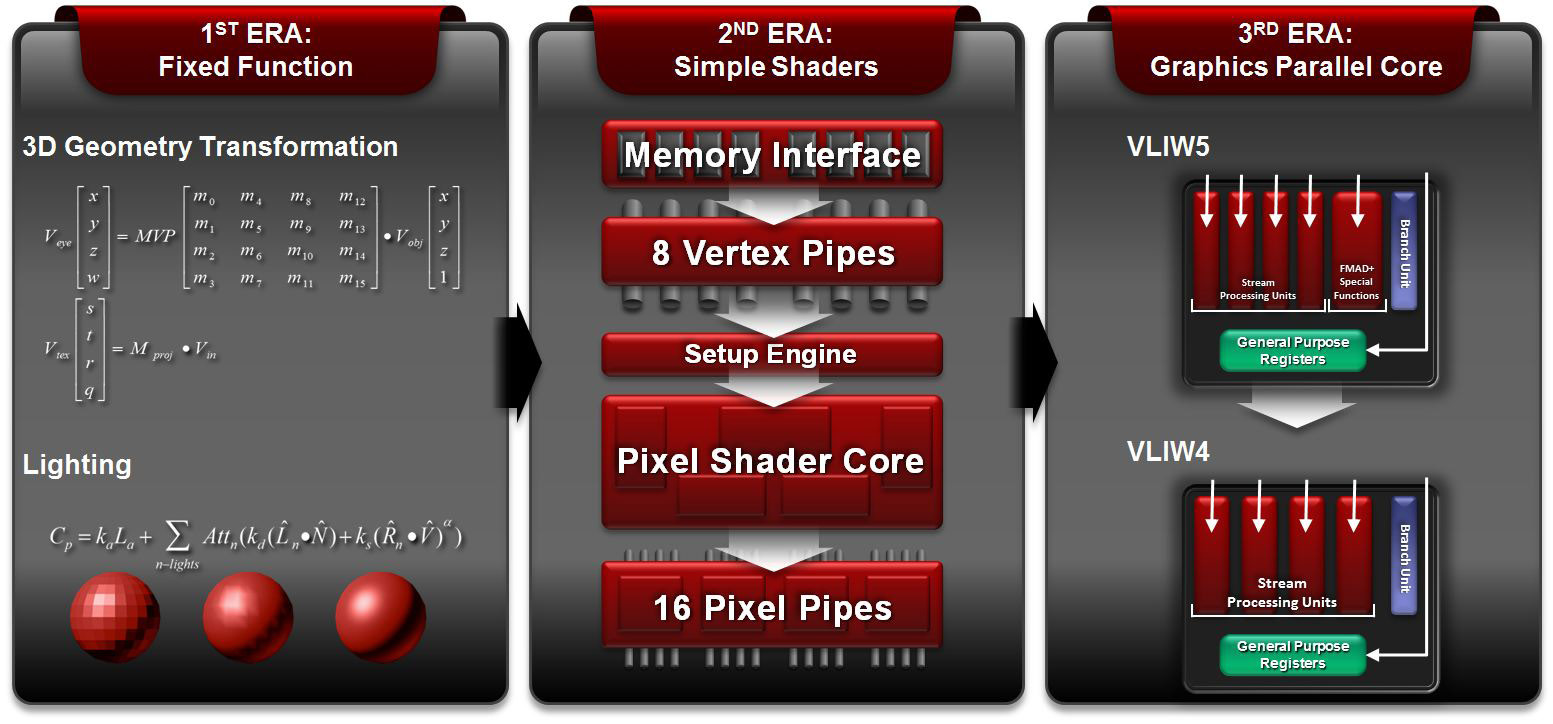
\includegraphics[width=10cm,keepaspectratio]{pics/gpu/gpu_amdevoluce}
	\end{figure}
\end{frame}

\begin{frame}
\frametitle{GPU vs CPU}
  \scriptsize

	\begin{itemize}
	\item CPU - small number of very fast computing units.
	\item Large caches, large control, out-of-order instruction execution, ...
	\item GPU - large number of not that fast computing units, simpler units.
	\item Smaller caches, small control, more transistors allocated for computation, ...
  \item GPU - data parallel, semi tast parallel
  \item CPU - tast parallel, semi data parallel
	\end{itemize}

	\begin{itemize}
	\item CPU - málo, velmi výkonných výpočetních jednotek
	\item Velká keš, velké řízení, vykonávání instrukcí mimo pořadí, ...
	\item GPU - velké množství méně výkonných, jednodušších výpočetních jednotek
	\item Malé keše, malé řízení, víc tranzistorů pro výpočty, ...
  \item GPU - data parallel, náznak task parallel
  \item CPU - tast parallel
	\end{itemize}
	\begin{figure}[h]
	
\includegraphics[width=10cm,keepaspectratio]{pics/gpu/gpu_gpuvscpu.pdf}
	\end{figure}
\end{frame}

\begin{frame}
\frametitle{GPU vs CPU}
	\begin{figure}[h]
	
\includegraphics[width=10cm,keepaspectratio]{pics/gpu/gpu_common}
	\end{figure}
  \scriptsize

	\begin{itemize}
	\item GPU is composed from multi-processors and device memory.
  \item Nvidia - streaming multi processor (SM).
  \item AMD   - compute unit (CU).
  \item Multi-processor is composed of SIMD units and various kings of memory.
  \item Computation executed on one multi-processor is independed from computation on other multi-processors.
  \item SIMD cores are commony reffered as shader unit (AMD Radeon HD7970M 20xCU, 64 shader unit per CU, = 1280 shader unit).
	\end{itemize}

	\begin{itemize}
	\item Grafická karta je složena z několika multiprocesorů a grafické paměti.
  \item Nvidia - streaming multi processor (SM).
  \item AMD   - compute unit (CU).
  \item Tento multiprocessor je dále složen z velkého množství jader a různých druhů pamětí.
  \item Akce, která beží na jednom multiprocesoru je nezávislá na akci, která běží na jiném multiprocesoru.
  \item Jádra bývají označována jako shader unit (AMD Radeon HD7970M 20xCU, 64 shader unit na CU, = 1280 shader unit).
	\end{itemize}
\end{frame}

\begin{frame}
\frametitle{NVIDIA - GTX 1080}
	\begin{figure}[h]
	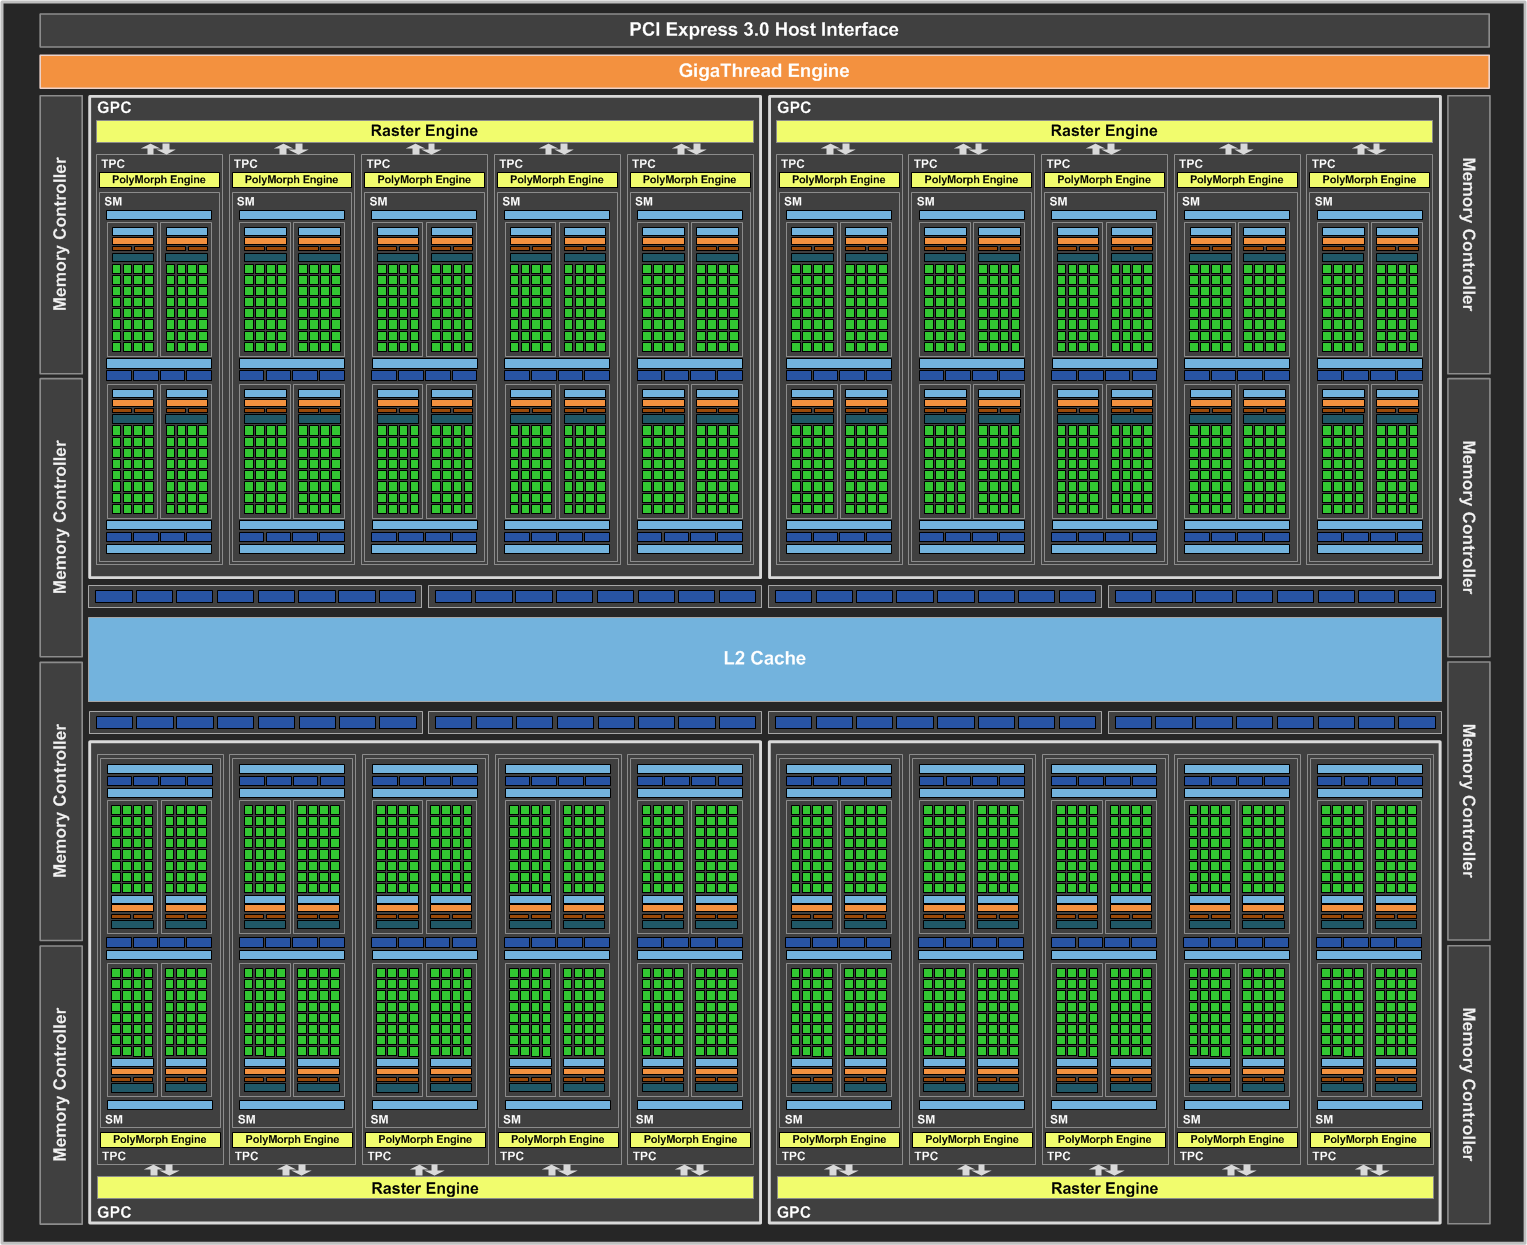
\includegraphics[width=8.5cm,keepaspectratio]{pics/gpu/1080}
	\end{figure}
\end{frame}

\begin{frame}
\frametitle{AMD FuryX/fiji}
	\begin{figure}[h]
	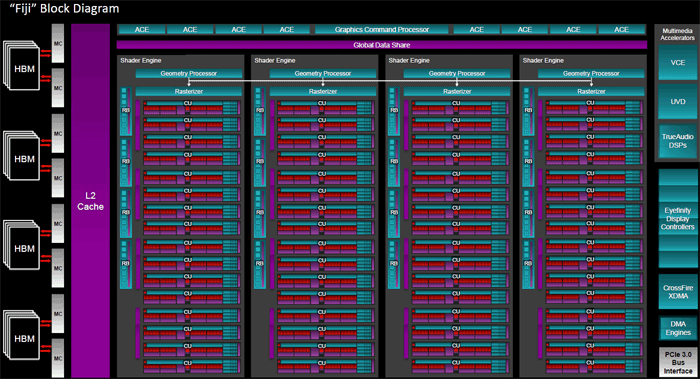
\includegraphics[width=11cm,keepaspectratio]{pics/gpu/furyx}
	\end{figure}
\end{frame}

\begin{frame}
\frametitle{NVIDIA - Fermi SMX}
	\begin{figure}[h]
	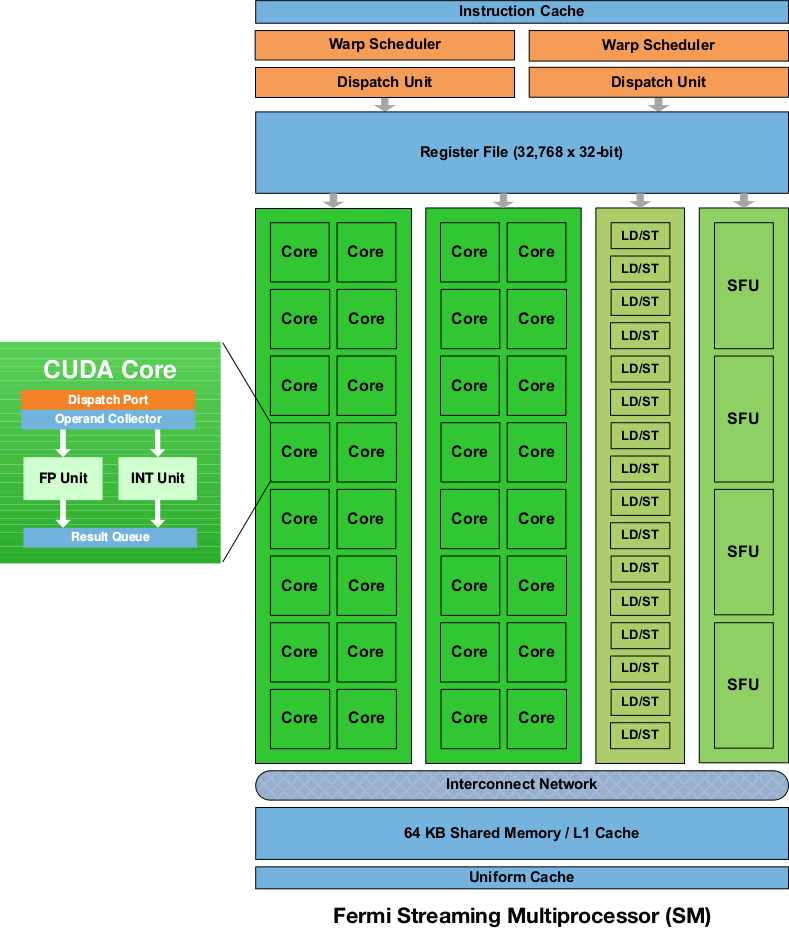
\includegraphics[width=7cm,keepaspectratio]{pics/gpu/fermi}
	\end{figure}
\end{frame}

\begin{frame}
\frametitle{NVIDIA - 1080 SMX}
	\begin{figure}[h]
	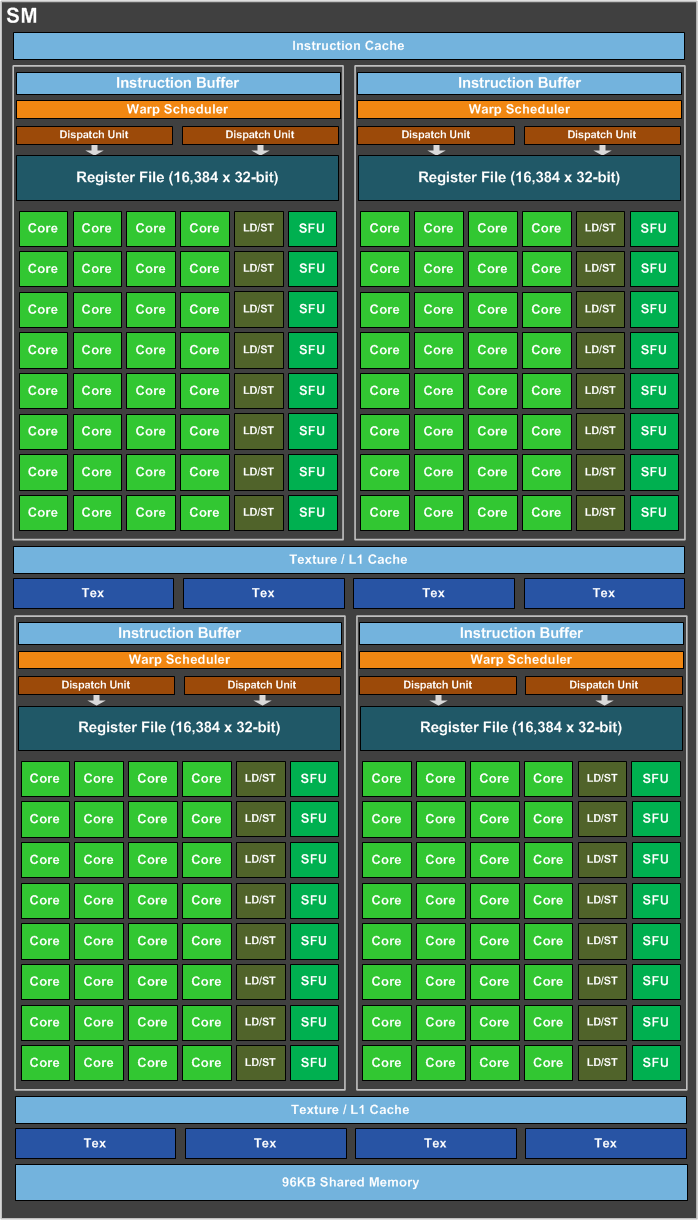
\includegraphics[width=4.5cm,keepaspectratio]{pics/gpu/1080SMX}
	\end{figure}
\end{frame}

\begin{frame}
\frametitle{AMD - GCN}
	\begin{figure}[h]
	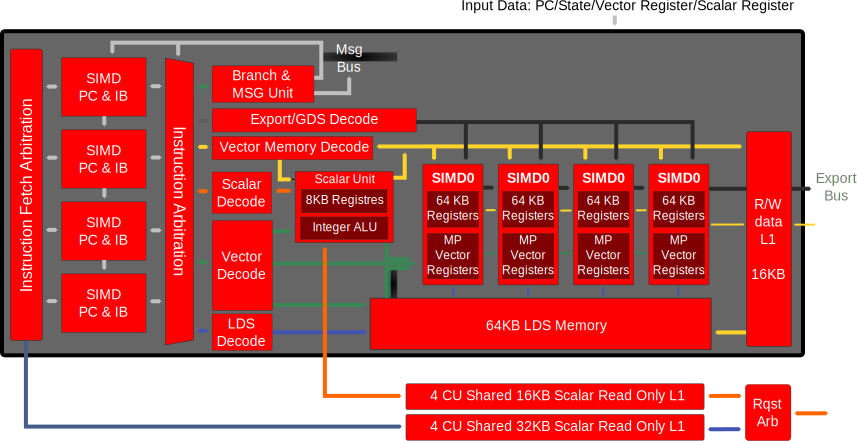
\includegraphics[width=11cm,keepaspectratio]{pics/gpu/gcn}
	\end{figure}
\end{frame}

\begin{frame}
\frametitle{Non programable parts of GPU / Hardwarové části}
  \scriptsize
	\begin{itemize}
	\item Today's GPUs are highly programable.
  \item Few parts remain fixed for configurable.
  \item Rasterization - converting vector primitives to fragments.
  \item Tessellation - splitting polygons into many sub-polygons.
  \item Texture units - filtering, wraping, compression, ...
  \item Per-fragment-operation, depth buffer, stencil buffer, ...
  \item Ray-tracing, ...
  \item And more
  \item Some parts are inaccessible from some APIs (CUDA cannot use rasterization).
	\end{itemize}
	\begin{itemize}
	\item Dnešní GPU jsou značně programovatelné
  \item Některé části stále zůstávají hardwarově zadrátované
  \item Rasterizace - převod trojúhelníků na fragmenty
  \item Tessellace - rozřezání polygonů na mnoho podpolygonů
  \item Texturovací jednoty - filtrování, opakování na okrajích, ...
  \item Depth buffer, Stencil buffer, ...
  \item A další
  \item Ke většině lze přistoupit pouze z některých API (OpenGL, Vulkan, DirectX)
	\end{itemize}
\end{frame}

\begin{frame}
  \frametitle{Memory Hierarchy / Paměťová hierarchie}
  \begin{columns}[T]
    \begin{column}{.48\textwidth}
      \begin{figure}[h]
        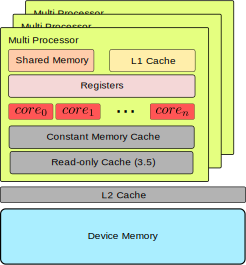
\includegraphics[width=5cm,keepaspectratio]{pics/gpu/memory_hierarchy}
      \end{figure}
    \end{column}
    \begin{column}{.48\textwidth}
      \scriptsize
      \begin{itemize}
        \item Different memory types with different size and speed.
        \item General rule: closer to core, faster, smaller memory.
        \item Registers are fastest (Ada contains 256KB of registers per SM).
        \item Shared/Local memory is used for thread communication.
        \item Device memory/global memory is cached using L2 cache. Large, big latency (100s of clocs).
      \end{itemize}

      \begin{itemize}
        \item Spousta různých pamětí s různou velikostí a rychlostí.
        \item Obecně platí, čím blíže k jádru, tím rychlejší a tím menší.
        \item Registry jsou nejrychlejší (na Ada je 256KB registrů na SM).
        \item Sdílená paměť slouží pro komunikaci mezi vlákny.
        \item Device memory (global memory) je velká (16GB i více), ale pomalá paměť.
      \end{itemize}
    \end{column}
  \end{columns}
\end{frame}

\begin{frame}
  \frametitle{Thread Hierarchy / Vláknová hierarchie}
  \scriptsize
  \begin{itemize}
    \item Thread is kernel instantion with unique index.
    \item Kernel/Shader is program composed of instruction.
    \item User launches 1000s of threads - Dispatch.
    \item Dispatch is divided into work-groups. Whole work-group runs on one SM.
    \item WG are further divided into Warps/Wavefronts (32/64 threads sub-groups).
    \item Warps/Wavefronts are executed on SIMD unit. (One warp per one SIMD).
    \item Threads in WG can be synchronized and can use shader memory.
    \item WG are 1D, 2D, 3D (dictates thread ordering and indices).
    \item Terminology differs (OpenCL, Cuda, Compute Shader, ...).
  \end{itemize}
  \begin{itemize}
    \item Na GPU pouštíme instance kernelů - vlákna.
    \item Kernel je program složený z instrukcí (podobně jako shader) a běží ve vláknu.
    \item Instrukce v kernelu jsou spouštěny v mnoha instancích na jádrech SM.
    \item Vlákna (thread, invocation, work-item) jsou seskupovány do pracovních skupin (work-group).
    \item Vlákna v pracovních skupinách můžou být na sobě závislá.
    \item Skupiny můžou být 1D, 2D, 3D (určuje pořadí vláken a jejich index).
    \item Mnoho work-group tvoří dispatch (taky může být 1D, 2D, 3D).
    \item Terminologie se liší (OpenCL, Cuda, Compute Shader, ...).
  \end{itemize}
\end{frame}

\begin{frame}
  \frametitle{Compute shader}
  \begin{picture}(320,250)
		\put(-28,50){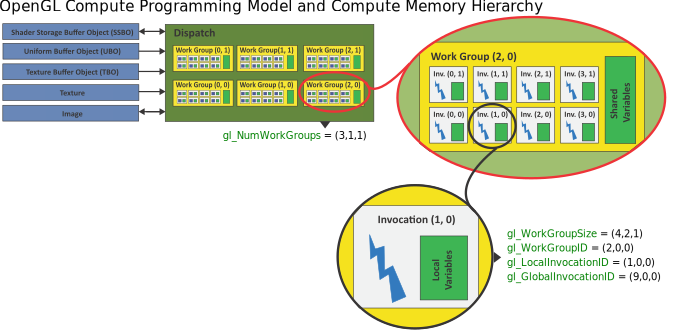
\includegraphics[height=6.4cm]{pics/gpu/threadHierarchy}}
	\end{picture}
\end{frame}

\begin{frame}
  \frametitle{Thread Hierarchy / Vláknová hierarchie}
  \begin{figure}[h]
	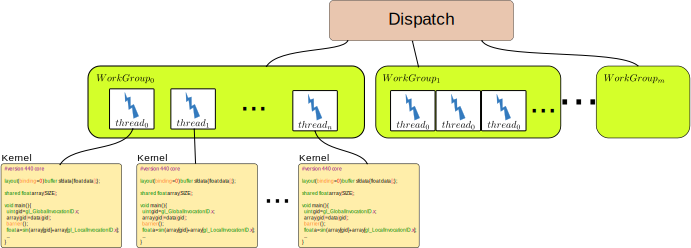
\includegraphics[width=11cm,keepaspectratio]{pics/gpu/thread_hierarchy}
	\end{figure}
  \scriptsize

  \begin{itemize}
    \item Threads are grouped to work-groups.
    \item Work-group can be 1D, 2D, 3D.
    \item WG are grouped into dispatch.
    \item Dsipatch can also be 1D, 2D, 3D.
    \item One SM can lauch multiple work-groups, if there is enough resourses (registers, shader memory).
  \end{itemize}

  \begin{itemize}
    \item Vlákna jsou seskupena do skupin work-group.
    \item Work-group může být 1D, 2D, 3D.
    \item Work-groupy jsou seskupeny do dispatch.
    \item Dispatch může být také 1D, 2D, 3D.
    \item Na jeden SM se může pustit vícero Work-group, pokud na to vystačí zdroje (registry, sdílená paměť)!
  \end{itemize}
\end{frame}

